\documentclass[letterpaper]{article}

\usepackage{outline}
\usepackage{graphicx}
\usepackage{listings}

\lstset{numbers=left, basicstyle=\footnotesize}

\begin{document}

\title{Implementing Distributed Systems Directly with I/O Automata in Ioa++}
\author{Justin R. Wilson \and Christopher D. Gill}
\date{}

\maketitle

\begin{abstract}
The ability to realize sophisticated distributed systems such as those found in cyber-physical, pervasive, or enterprise computing environments is predicated on a suitable model and implementation of asynchrony and concurrency.
The size and complexity of these systems implies that software re-use in their development, maintenance, and evolution is also essential.
Taken together, these requirements demand appropriate programming abstractions through which different forms of asynchrony and concurrency can be realized directly and easily in reusable software.
% By ``different forms'' we mean single-threaded, multi-threaded, time triggered, event triggered, etc.

To that end, this paper presents the \emph{ioa++ framework} for developing distributed systems, which is the primary contribution of this research.
We outline a system model for asynchronous and concurrent systems, which is grounded in the design and implementation of the I/O automata formal model.
We describe the design and implementation of ioa++ and show how ioa++ can be used to develop a real network protocol.

Our experiences demonstrate that ioa++ can help simplify developing distributed systems, by supporting reasoning about asynchronous and concurrent programs directly from the source code using the I/O automata formal model.
Common concurrency and interaction semantics allow simple modules to be aggregated into complex systems without building adapters that convert from one thread model or event system to another.
Whereas reasoning about the correctness of modules in a threaded program requires considering interactions among the various threads, reasoning about the correctness of modules in ioa++ is limited to the modules themselves and a well-defined set of composition rules.

We evaluate the ability to concurrently execute actions in ioa++ through a series of micro-benchmarks which confirm that concurrent execution is limited by the interactions of the automata that comprise the system and the overhead of synchronization.
\end{abstract}


\section{Introduction}

Advances in embedded systems and networking are paving the way for distributed systems of unprecedented sophistication.
Cyber-physical systems go beyond the traditional embedded system paradigm by explicitly modeling the dynamics of the physical system and communication network in the computational task.
The inclusion of wireless network interfaces in modern electronic devices is transforming our homes, offices, and hospitals into pervasive computing environments.
The interactions these systems have with the physical environment and its community of users require a degree of interoperability, configurability, adaptability, scalability, robustness, and security not found in existing systems.

One of the forces that prevents the development of any kind of sophisticated software system is accidental complexity~\cite{brooks_nsb}.
In the context of distributed systems, a major source of accidental complexity is a mismatch between the conceptual model of the system and the technology used to implement the system.
The mismatch between the conceptual model and implementation method introduces defects due to translation errors, slows rapid prototyping, and retards iterative refinement.
While there is no ``silver bullet''~\cite{brooks_nsb}, reducing the accidental complexity derived from the mismatch between concept and implementation will increase productivity and make new levels of sophistication possible with existing levels of effort.

Threads are the de facto implementation vehicle for most of computing including distributed systems.
Threads dominate because modern processors, programming languages, and operating systems were all developed to support the thread model.
Furthermore, the widespread availability of thread libraries makes them a natural choice for system development.
While threads dominate in practice, using threads to develop systems has a number of significant drawbacks.

First, ad hoc communication among threads prohibits software reuse.
To illustrate this problem consider the challenge of developing an application with a graphical user interface that also uses a multi-threaded middleware library.
Graphical user interfaces often use a single-threaded event-based design, e.g., X, Swing.
The system integrator must write glue code that bridges the single-threaded event-based semantics to multi-threaded semantics.
Bridging between two thread models is achievable, however, the systems we desire to build will rely on many libraries each with their own thread model.
The importance of a unified approach to concurrency becomes apparent when one considers bridging between different threading models, e.g., event-based, reactor, proactor, active objects, and their attributes, e.g., priority, thread-creation, blocking vs. non-blocking I/O.

Second, threads are difficult to treat formally and therefore \emph{very} difficult to treat informally.
The correctness of programs is reasoned about either formally as part of formal software design and verification and/or informally during the debugging process.
Since most programs will never be formally verified, the correctness of most programs hinges solely on the developers ability to reason about the program.
Based on the historical example of structured programming~\cite{goto_considered_harmful}, there is a strong correlation between what is ``easy'' in the formal arena and what is ``easy'' in the informal arena, especially when the implementation mimics the formal model, e.g., structured programming languages.
It is well known that a formal treatment of threads is difficult due to the arbitrary interleaving of critical sections and ability to define critical sections of arbitrary scope~\cite{lee_threads}.
Thus, the correctness of most multi-threaded programs hinges on the developer's ability to explore arbitrary interleavings of critical sections, i.e., model checking, in their head.

Third, threads are ill-suited for the asynchronous semantics present in the systems we desire to build.
The distributed systems we desire to build are asynchronous at both the device and network levels.
Embedded devices must respond to asynchronous events in the environment.
The interrupt-driven TinyOS operating system for wireless sensor network motes is an exemplar in this area.
The fundamental communication primitive in real-world distributed systems is asynchronous message passing.
Realizing asynchrony in a threaded program requires the use of signals (interrupts) and/or (a)synchronous I/O multiplexing.
Signals are primitive, rigid, and difficult to use correctly.
Synchronous I/O multiplexing, e.g., a select loop, is limited to operating system abstractions, e.g., file descriptors, and induces a reactive state machine structure that is difficult to understand and maintain.
Asynchronous I/O improves efficiency by avoiding the dispatching necessary to determine the I/O operation but are subject to the same limitations of shared-state thread-based programming.

Difficulties in developing asynchronous and concurrent software using threads has prompted a number of concurrent programming languages, e.g., Esterel, Erlang, Ptolemy, Autopipe, and language extensions, e.g., OpenMP, Cilk, Split-C.
Solutions that involve creating a new language or extending an existing language suffer from two main problems.
First, such solutions are often domain-specific and do not generalize to different applications, a necessity for heterogeneous distributed systems.
Furthermore, solutions not connected to a general-purpose formal model lack the important property that the complete system including the environment can be modeled as another component.
Second, such solutions often fail to become mainstream due to practical considerations.
For example, the combination of C and pthreads is much more popular than Erlang due to the popularity of C-like languages and C's connection with UNIX operating system.
Most language extensions are targeted at niche markets and therefore never standardized and implemented in mainstream compilers.

Thus, in order to build sophisticated distributed systems, we require a common semantics and model for building concurrent and asynchronous systems with straight-forward abstractions.
%% The model must be general to support the wide variety of devices and protocols necessary for cyber-physical and pervasive computing systems.
%% The model must facilitate the development of concurrent modules that can be reused.
%% The model must have a strong connection with a formal model to simplify the task of reasoning about individual components and complete systems.
%% The model must be implemented in such a way that it is easily approachable.
In section~\ref{system_model}, we expound upon the requirements of the model and connect the requirements with the I/O automata formal model.
Section~\ref{representation} describes how I/O automata are represented in our I/O automata framework.
In section~\ref{design}, we describe the design and implementation of our I/O automata framework.
Section~\ref{evaluation} provides an evaluation and discussion of our framework.
Section~\ref{related_work} contains an overview of related work and we offer our conclusions and thoughts for future work in section~\ref{conclusion}.

%% We provide a common semantics and model for building concurrent and asynchronous systems with straight-forward abstractions.

%%formal models, e.g., UNITY, I/O Automata,

%% Devices are asynchronous and concurrent.
%% Networks are asynchronous and concurrent.
%% Why not start with a model that is asynchronous and concurrent?

%% What inspires us:
%% \begin{itemize}
%%   \item CORBA - Remote Method Invocation (Remote Procedure Call with a ``this'' pointer).
%%     ``Let's make synchronous function calls over a network.''
%%     Assumes a thread of control.
%%     Asynchronous calls were added later (Did these result in obfuscation?)

%%   \item Patterns for asynchronous concurrency in a synchronous, thread-based world: Active objects, Reactor, Proactor, etc.
%%     Examples: X server, OS2 Presentation Manager, Java Swing

%%   \item AJAX - The modern Web is built on JavaScript + \emph{asynchronous} web page requests = AJAX.

%%   \item Michi Henning - ICE

%%   \item Steve Vinoski - Toolbox of programming languages

%% \end{itemize}

%% We provide a common semantics and model for building concurrent and asynchronous systems with straight-forward abstractions.


\section{I/O Automata Component Model\label{component_model}}

%% Modularity, well-defined interfaces, and composition are essential properties of reusable software.
%% A unit of software that exhibits all of these properties is called a \emph{component}~\cite{szyperski2002component}.
%% Modularity implies that a component can be deployed independently of other components.
%% Well-defined interfaces and interactions allow components to expose their functionality in a regular way that facilitates reasoning about different interactions among them.
%% Composition allows a group of interacting components to be understood as a cohesive unit.

In this section we describe how the I/O automata model offers a natural realization of components and interfaces, and provides natural support for concurrency and composition.
%% We then describe extensions to support dynamic semantics as participants in the system may arrive and depart at run-time.
We then describe extensions to support semantics for \emph{dynamic systems,} i.e., systems whose set of constituent automata changes over time.

\paragraph*{I/O automata.}
The Input/Output (I/O) automata model was developed to model reactive concurrent and asynchronous systems~\cite{lynch1996distributed}.
An I/O automaton consists of state variables and a set of atomic actions that manipulate the state variables.
An action is only permitted to manipulate the state variables of the automaton to which it belongs.
An action is either an internal action, an output action, or an input action.
An internal action only changes the state of the automaton.
An output action changes the state of the automaton and produces a signal or value that may be consumed by one or more input actions.
An input action changes the state of the automaton when it receives a signal or value produced by an output action.
\ifjournal
The set of actions associated with an automaton is known as the automaton's \emph{signature}~\cite{lynch1996distributed}.
\fi
\ifjournal
Often, a local action consists of a precondition and an effect.
The precondition is a predicate over the state variables that enables the effect when selected for execution.
The effect is a function that computes the next state of the automaton from the current state.
An input action presented in this style consists solely of an effect.
\fi
I/O automata are \emph{composed} by (1)~concatenating the state variables of the constituent automata, (2)~consolidating the effects of all input actions with the same name, and (3)~incorporating the effects of input actions into output actions with the same name.
Execution in the I/O automata model consists of non-deterministically and repeatedly selecting a local action (an output or internal action~\cite{lynch1996distributed}) and then if the precondition is true applying the effect.
The scheduler is assumed to be \emph{fair,} meaning that a local action is guaranteed to be selected (but not necessarily executed) infinitely often.

\begin{figure*}
\center
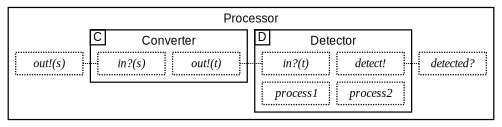
\includegraphics[width=\textwidth]{system_model}
\caption{Example event detection system.}
\label{sys_model}
\end{figure*}

\paragraph*{Motivation for I/O automata based components.}
%The I/O automata formalism was developed to model reactive systems~\cite{lynch1987hierarchical} and has been used in the design and verification of concurrent and distributed systems.
I/O automata are a good foundation for such components because they have independent state, straightforward interfaces, and precise semantics for event generation, distribution, and consumption resulting in well-defined interactions under composition.
\emph{Hierarchical decomposition} is an established technique for I/O automata~\cite{lynch1994atomic} which allows a \emph{parent} to contain zero or more \emph{children}.
The \emph{root automaton} is at the top of the hierarchy represents the entire system as composition is applied recursively upward.
To illustrate how components can be expressed naturally using I/O automata, Figure~\ref{sys_model} shows a simple event detector comprising three component automata: an anonymous Processor, a Converter named C, and a Detector named D. 
The Processor is the root and C and D are its children.
Automata are depicted as solid rectangles. The type of the automaton appears in a box in the upper left or lower left corner, e.g., Processor.
Actions are depicted as dotted rectangles and bindings are indicate by dotted lines with an arrow pointing to the input action.
Output actions are suffixed with \emph{!} (e.g., \emph{detect!}), input actions are suffixed with \emph{?} (e.g., \emph{detected?}), and internal actions have neither suffix (e.g., \emph{process1}).
The type associated with the value produced or consumed by an action is in parentheses after the name (e.g., \emph{out!(s)}).

\paragraph*{Explicit composition.}
Composition of I/O automata is based on actions having the same name.
To prepare for dynamic composition, we redefine composition at the action level.
An explicit association between an output action and input action is called a \emph{binding}.
%% The automaton that prescribes a binding is said to \emph{own} the binding.
%% A binding is denoted $(output, input, owner)$.
The set of bindings in a system must adhere to four essential rules.
First, the output action and input action of a binding must agree on the type being produced and consumed.
Second, an input action can be bound to at most one output action.
Third, an output action cannot be bound to more than one input action in the same automaton.
Fourth, an output action cannot be bound to an input action in the same automaton.
The second, third, and fourth rules prevent ambiguity in the relationship between the states of the associated automata.
Graphically, an arrow originating in one component automaton must terminate in another component automaton as Figure~\ref{sys_model} illustrates.
%% To adhere to this rule, the following must be true for the global binding map $B$:  $\langle \forall o, i : (o, i) \in B :: \pi (o) \neq \pi (i) \rangle$.

\paragraph*{Concurrent execution.}
Since each automaton is independent, opportunities exist for concurrent execution if the state of each automaton is preserved and a composition is not reduced to a single equivalent automaton.
Each local action implies a set of automata which in turn implies a set of state variables that might be modified.
For an internal action, this set consists of the automaton containing the internal action.
For an output action, this set consists of the automaton containing the output action and the automata that contain the input actions to which the output action is bound.
Two actions can be executed concurrently if their respective sets of state variables are disjoint.
The implied automata sets for each local action in Figure~\ref{sys_model} are: $out!(s) \to \{root, C\}$, $out!(t) \to \{C, D\}$, $process1 \to \{D\}$, $process2 \to \{D\}$, and $detect! \to \{D, root\}$.
Thus, $out!(s)$ and $process1$ can be executed concurrently while $process1$ and $detect!$ can not.

\ifjournal
These observations create some interesting opportunities for designing and analyzing concurrent software.
Migrating intense computation to internal actions increases the level of parallelism in a system, i.e., the set of implied automata is small.
A high degree of fan-out (an output action being bound to many input actions) creates a bottle-neck and decreases the level of parallelism, i.e., the set of implied automata is large.
However, the input effects can be applied in parallel since the state of each automaton is independent.
A high degree of fan-in (an automaton has many bound input actions) also creates a bottle-neck by increasing the probability that two sets of implied automata will not be disjoint.
A scheduler might cluster and pin automata to processors to maximize concurrent execution while minimizing inter-processor communication.
Compositions of automata can be statically composed to take advantage of in-lining.
An individual automaton can be decomposed into a number of child automata to increase parallelism.

\paragraph*{Parameters and action types.}
Actions in the I/O automata model can be defined using parameters.
Parameters are useful for situations requiring fan-in or session semantics.
For example, consider an automaton with an input action $in?(s)$ that is to be bound to $N$ different output actions.
To get around the limitation that an input can only be bound to one output, we augment the input action with a parameter that indicates the associated output action, e.g., $in?[i](s)$ where $i$ takes on the integer values from 1 to $N$.
\emph{Parameterized} actions take a parameter while \emph{unparameterized} actions do not.
Parameters, for actions that require them, are specified in the binding and serve to identify the action.

\emph{Unvalued} output and input actions produce and consume signals respectively.
\emph{Valued} output and input actions produce and consume values respectively.
The allowed combinations of input, output, and internal actions, unvalued and valued actions, and unparameterized and parameterized actions result in 10 possible action types:
unvalued unparameterized output (uv-up output),
unvalued parameterized output (uv-p output),
valued unparameterized output (v-up output),
valued parameterized output (v-p output),
unvalued unparameterized input (uv-up input),
unvalued parameterized input (uv-p input),
valued unparameterized input (v-up input),
valued parameterized input (v-p input),
unparameterized internal (up internal), and
parameterized internal (p internal).

\begin{figure}
\center
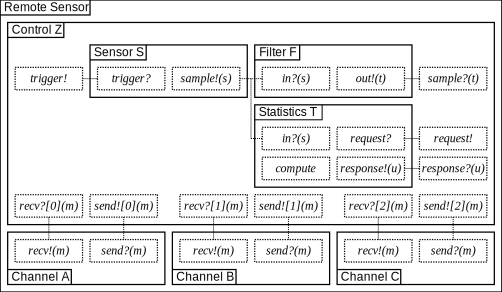
\includegraphics[width=\columnwidth]{example1}
\caption{Example remote sensor system.}
\label{example1}
\end{figure}

\paragraph*{Example.}
Figure~\ref{example1} depicts a remote sensor system as a composition of automata using a scheme similar to Figure~\ref{sys_model} where parameters are given in brackets after the action name, e.g., \emph{recv?[0](m)}.
The Remote Sensor automaton consists of the Control automaton Z and three Channel automata A, B, and C representing three network connections.
The Control automaton Z consists of the Sensor automaton S, the Filter automaton F, and the Statistics automaton T.
The Control automaton C starts the sampling process with the uv-up output $Z.trigger!$.
The uv-up input $S.trigger?$ is executed atomically with $Z.trigger!$ due to the binding $(Z.trigger!, S.trigger?)$.
When the sampling process is complete, the v-up output $S.sample!(s)$ distributes the sample to the Filter F and Statistics component T via the $(S.sample!(s), F.in?(s))$ and $(S.sample!(s), T.in?(s))$ bindings.
Note that $S.sample!(s)$, $F.in?(s)$, and $T.in?(s)$ all agree on the type of the sample $s$.
The Filter automaton F passes the filtered sample to the Control automaton Z via the $(F.out!(t), Z.sample?(t))$ binding.
The Statistics automaton T calculates the statistics incrementally using the up internal $T.compute$.
The statistics can be polled by the Control automaton Z by issuing a request via the $(Z.request!, T.request?)$ binding and then receiving a response via the $(T.response!(u), Z.response?(u))$ binding.
The Control automaton Z contains a vp-output $Z.send![](m)$ and a vp-input $Z.recv?[](m)$ for sending and receiving network messages using the Channel automata A, B, and C.
The parameters 0, 1, and 2, are used to route messages to Channel automata A, B, and C respectively using the session idea mentioned previously.
Opportunities for concurrent execution exist for the remote sensor depicted in Figure~\ref{example1}.
The set of automata implied by $Z.trigger!$ is $\{Z, S\}$ while the set of automata implied by $T.compute$ is $\{T\}$.
Since the sets are disjoint, the two actions can be executed concurrently.
\fi

%% \subsection{Practical Considerations\label{practical}}

%% As a mathematical abstraction the I/O automata model is appropriate for modeling reactive asynchronous and concurrent systems.
%% However, it lacks certain features needed to develop real components.
%% This subsection introduces these features and lays the foundation for adding the dynamics discussed in Section~\ref{dynamics}.

%% The I/O automata model assumes that systems are composed of a finite or countably infinite number of automata~\cite{lynch1996distributed}.
%% Assuming a countably infinite number of participants allows properties of the systems to be stated in terms of an abstract quantity representing the number of members, e.g., $N$, and is reasonable because all real systems are composed of a finite number of members.
%% The set of interactions in the I/O automata model is also fixed since automata are statically composed.
%% Dynamic systems can be \emph{modeled} in that approach by assuming that only a subset of the all the automata that could possibly exist are actively participating in the system.
%% To use this technique, a flag is associated with each automaton indicating if it is active or inactive and external actions for activation and deactivation are defined~\cite{lynch1994atomic}.

%% \paragraph*{Limitations of the static model.}
%% While assuming a fixed number of automata is reasonable for modeling, assuming a fixed number of automata for a real system may result in either over-provisioning or inflexibility.
%% To develop a component based on the static I/O automata model, a developer must choose a concrete value for the abstract quantity $N$.
%% System resources are wasted if the actual number of participants is much smaller than $N$.
%% If the number of participants is greater than $N$, then the system cannot respond to certain situations even though resources might be available.
%% Thus, the techniques for \emph{modeling} a dynamic system of I/O automata are not necessarily appropriate for \emph{implementing} a dynamic system of I/O automata.
%% %% Consequently, we add the ability to deal with a dynamic set of automata and interactions.

%% To illustrate, let a system $S=(A,B)$ be a pair consisting of a set of automata $A$ and a set of bindings $B$.
%% The I/O automata model assumes that $S$ and therefore $A$ and $B$ are both fixed, so that dynamics must be \emph{simulated} via the manipulation of activation flags.

\paragraph*{Support for dynamic systems.}
The I/O automata model assumes that systems are composed of a finite or countably infinite number of automata~\cite{lynch1996distributed} and models dynamic systems by activating and deactivating automata as appropriate~\cite{lynch1994atomic}.
While appropriate for modeling, this assumption is not conducive to building flexible and efficient systems because it requires \emph{a priori} bounds on all resources.
To address the limitations of the static representation of dynamic systems, ioa++ provides architectural support for dynamic systems by separating the concerns of \emph{enacting} versus \emph{initiating} actions for managing dynamics into distinct \emph{system} and \emph{base} automata respectively.
We define four \emph{system actions} for managing dynamic systems of automata: \emph{create}, \emph{bind}, \emph{unbind}, and \emph{destroy}.
The \emph{create} action allows an automaton to create a child automaton.
The \emph{bind} action allows an automaton to associate an input action with an output action while the \emph{unbind} action allows an automaton to dissociate an input action from an output action.
The \emph{destroy} action allows an automaton to destroy a child automaton and all bindings associated with it (recursively).

\begin{figure*}
\center
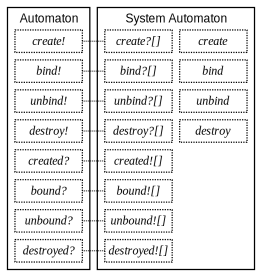
\includegraphics[width=\textwidth]{system_action}
\caption{System automaton and actions.}
\label{system_action}
\end{figure*}
% A dynamic system implies that the system $S$ must be dependent on time $t$ as a function of the number of actions that have been executed by $t$.
% Thus, $S_{t+1}$ need not be equal to $S_{t}$.
% A \emph{system action} is an action that \emph{can} change the system $S$.
% The set of automata $A$ and set of bindings $B$ are managed by the \emph{system automaton} which represents the run-time system.
As Figure~\ref{system_action} illustrates, the system automaton provides: parameterized input actions for receiving requests to create, bind, unbind, and destroy automata; internal actions for evaluating and enacting system action requests; and corresponding parameterized output actions for returning responses to system action requests.
(Parameterized actions are indicated with [].)
The base automaton provides output actions that trigger requests to create, bind, unbind, and destroy automata, along with
input actions to receive the results.
User-defined component automata (i.e., \emph{user automata}) inherit from the base automaton.
Each user automaton is thus composed (not bound) with the system automaton and inherits output actions for requesting system actions and input actions for receiving the results of system actions.

%% Let $A$ be the set of automata that exist where each element in $A$ is a pair $(p, a)$ where $p$ is the parent of $a$.
%% Let $B$ be the set of bindings that exist where each element in $B$ is a tuple $(w, o_a, o_n, o_p, i_a, i_n, i_p)$ where $w$ is the automaton that owns the binding, $o_a$ is the output automaton, $o_n$ is the name of the output action, $o_p$ is the parameter of the output action, $i_a$ is the input automaton, $i_n$ is the name of the input action, and $i_p$ is the parameter of the input action.
%% Define the predicate $exists (a) = \langle \exists p, q : (p, q) \in A :: q = a\rangle$ that is true when automaton $a$ exists, i.e., has a parent\footnote{The root automaton's parent is the special symbol $\perp$.}.
%% Define the predicate $existsb (a) = \langle \exists a : (w, o_a, o_n, o_p, i_a, i_n, i_p) \in B :: a = w \lor a = o_a \lor a = i_a \rangle$ that is true when automaton $a$ appears somewhere in $B$.
%% We define the create operation as the Hoare triple $\{exists (p) \land \lnot exists (a)\} \quad create(a)_p \quad \{(p,a) \in A\}$ which says that the parent automaton $p$ can create automaton $a$ if $p$ exists and $a$ does not exist.
%% The destroy operation can be defined $\{(p,a) \in A\} \quad destroy(a)_p \quad \{(p,a) \notin A \land \lnot existsb(a)\}$ which says that in order to destroy $a$ and remove all bindings associated with $a$, $p$ must be the parent of $a$.
%% Define the predicate $free (a, n, p) = \langle \forall w, o_a, o_n, o_p, i_a, i_n, i_p : (w, o_a, o_n, o_p, i_a, i_n, i_p) \in B :: \lnot (i_a = a \land i_n = n \land i_p = p) \rangle$ that is true when the input action argument is not bound.
%% Define the predicate $involved (o, n, p, i) = \langle \exists w, o_a, o_n, o_p, i_a, i_n, i_p : (w, o_a, o_n, o_p, i_a, i_n, i_p) \in B :: o_a = o \land o_n = n \land o_p = p \land i_a = i \rangle$ that is true when automaton $o$'s output action $(n, p, i)$ is bound to some input action in automaton $i$.
%% The bind operation can be defined $\{exists (w) \land exists (o_a) \land exists (i_a) \land free (i_a, i_n, i_p) \land \lnot involved(o_a, o_n, o_p, i_a) \land o_a \neq i_a \} \quad bind (w, o_a, o_n, o_p, i_a, i_n, i_p) \quad \{(w, o_a, o_n, o_p, i_a, i_n, i_p) \in B\}$ which says that in order for the binding to succeed the owner $w$ exists, automaton $o_a$ exists, automaton $i_a$ exists, the input action $(i_a, i_n, i_p)$ must not be bound, the output action $(o_n, o_p)$ of automaton $o_a$ cannot be bound to an input action in automaton $i_a$, and the automata $o_a$ and $i_a$ cannot be the same.
%% The precondition for $bind$ is same as the binding rules derived in Section~\ref{system_model} augmented with existence tests for the owner, output automaton, and input automaton.
%% The unbind operation is similar to destroy: $\{(w, o_a, o_n, o_p, i_a, i_n, i_p) \in B\} \quad unbind (w, o_a, o_n, o_p, i_a, i_n, i_p) \quad \{(w, o_a, o_n, o_p, i_a, i_n, i_p) \notin B\}$.

% I didn't do more complex transactions, i.e., create-and-bind, because its not clear how it fails.
% Are partial successes allowed?
% Furthermore, such  transactions can be arbitrarily complex which does not bode well for efficiency.

\paragraph*{Binding predicates.}
Consider a simple system consisting of two automata where automaton A reliably transfers messages to automaton B.
In a dynamic system, one cannot guarantee that the message will be received because there is no way to determine if the output action producing the message is bound to the input action receiving the message.
Since we can guarantee that the set of binding does not change during the execution of an action, we allow automata to query the current set of bindings using a \emph{binding predicate}.
Binding predicates are typically used the precondition of output actions to guarantee delivery.


\section{Design and Implementation\label{design}}

\begin{itemize}
  \item Problem
  \item Design forces
  \item Solution
  \item Consequences
\end{itemize}


\section{I/O Automata Programming Model\label{representation}}

In this section, we show how I/O automata can be used to construct programs.
To motivate the presentation, we develop an automaton for electing a leader in a unidirectional ring using the LCR algorithm.

\subsection{I/O Automata Representation}

\paragraph{Leader election in a unidirectional ring.}
Nodes in a distributed system are arranged in a ring so that two consecutive nodes are connected by a channel.
The goal is to designate one of the nodes as the leader of the ring.
The solution we adopt is the asynchronous LCR algorithm presented by Lynch in Chapter 15 of~\cite{lynch1996distributed} which is in turn based on the work of LeLann~\cite{le1977distributed} and Chang and Roberts~\cite{chang1979improved}.
The LCR algorithm assumes that every node has a unique identifier (UID).
When the protocol begins, each node sends its UID to its successor.
When a node receives a UID from its predecessor that is greater than its own UID, it forwards the UID to its successor.
When a node receives its own UID, it elects itself the leader of the ring.
Our implementation of the asynchronous LCR automaton is located in \verb+examples/asynch_lcr_automaton.hpp+ of the ioa++ package.

\paragraph{Declaring an automaton.}
All automata inherit from the common base class \verb+ioa::automaton+ which implements the system action interface.
The following code declares the \verb+asynch_lcr_automaton+:
\begin{lstlisting}
template <typename UID>
class asynch_lcr_automaton :
  public virtual ioa::automaton
{
  ...
};
\end{lstlisting}
Static composition can be accomplished by inheriting from, i.e., extending, other automata.
A problem arises when an automaton extends more than one automaton since the common \verb+ioa::automaton+ base class will be duplicated for each inheritance path.
The solution is to make the \verb+ioa::automaton+ base class a virtual base class which eliminates the duplicates and resolves all references appropriately.
The \verb+asynch_lcr_automaton+ is declared as a template where the type \verb+UID+ is the type used for unique identifiers.
This makes the \verb+asynch_lcr_automaton+ general since it can use any type that models the unique identifier concept.

\paragraph{Declaring and initializing state variables.}
The state variables of an automaton are expressed as member variables.
The \verb+asynch_lcr_automaton+ has four state variables containing the unique id of the automaton, a queue of outgoing messages, and flags for reporting a change in status:
\begin{lstlisting}
private:
  const UID m_u;
  std::queue<UID> m_send;
  bool m_report;
  bool m_leader;
\end{lstlisting}
Notice that the member variables are declared \verb+private+ which is in keeping with the notion that the state of each automaton is independent.
State variables are initialized using a constructor.
For the \verb+asynch_lcr_automaton+, the id is initialized, the send queue contains the id of the automaton, the automaton does not need to report its leader status, and the automaton is not the leader:
\begin{lstlisting}
public:
  asynch_lcr_automaton (const UID& u) :
    m_u (u),
    m_report (false),
    m_leader (false)
  {
    m_send.push (m_u);
    schedule ();
  }
\end{lstlisting}
The constructor also bootstraps the scheduler by scheduling all enabled local actions using the member function \verb+schedule+.
We will return to scheduling later in the discussion.

\paragraph{Declaring/defining actions.}
Actions are member variables that model the action concept.
An action has traits that indicate the type of action (input, output, internal), if the action is valued and the value type, and if the action is parameterized and the parameter type.
Actions also contain methods for preconditions, effects, and scheduling.
The traits are used to check that input actions are bound to output actions with the same value status and type and also control how the methods are executed.

To facilitate declaring actions, a number of wrappers and macros corresponding to the action types listed in section~\ref{practical} are available.
Local actions are declared using three functions corresponding to a precondition, effect, and scheduling call.
The macros assume the functions are named \verb+action_name_precondition+, \verb+action_name_effect+, and \verb+action_name_schedule+.
For example, the send action of the \verb+asynch_lcr_automaton+ is declared:
\begin{lstlisting}
private:
  bool send_precondition () const { ... }
  UID send_effect () { ... }
  void send_schedule () const { ... }
public:
  V_UP_OUTPUT (asynch_lcr_automaton, send, UID);
\end{lstlisting}
Input actions are declared similarly save the absence of a precondition.
The precondition and scheduling functions are not allowed to change the state of the automaton and are consequently declared \verb+const+.
The macros for actions that are subject to binding by other automata belong in a \verb+public+ section.

\paragraph{Scheduling.}
Automata subject actions to the scheduler using the \verb+ioa::schedule+ function.
A common pattern is to schedule all local actions using one function where each action is guarded by its precondition.
For the \verb+asynch_lcr_automaton+, the scheduling function is:
\begin{lstlisting}
  void schedule () const {
    if (send_precondition ()) {
      ioa::schedule (&asynch_lcr_automaton::send);
    }
    if (leader_precondition ()) {
      ioa::schedule (&asynch_lcr_automaton::leader);
    }
  }
\end{lstlisting}
The various scheduling functions in the \verb+asynch_lcr_automaton+ and the constructor all dispatch to this function.

\subsection{Dynamics}

\begin{figure}
\center
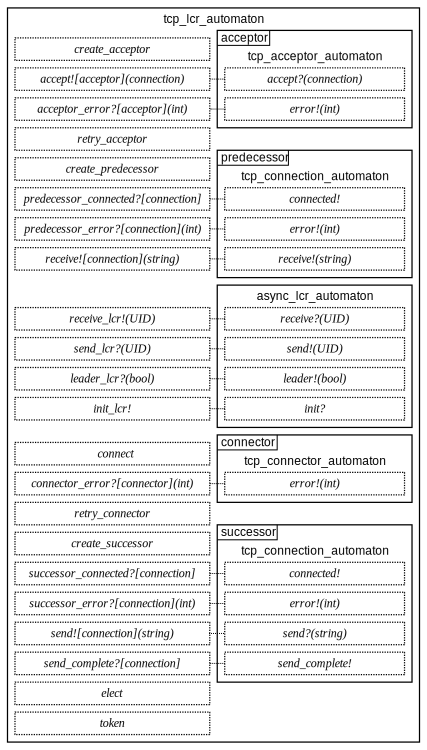
\includegraphics[width=\textwidth]{tcp_lcr_automaton}
\caption{TCP LCR automaton.}
\label{tcp_lcr_automaton}
\end{figure}

\paragraph{Leader election in a ring using TCP.}
The \verb+asynch_lcr_automaton+ is a reusable component designed to be used in the context of a larger system.
The \verb+tcp_lcr_automaton+ listed in \verb+examples/tcp_lcr.cpp+ elects a leader in a dynamic ring of processes.
The structure of the \verb+tcp_lcr_automaton+ is given in Figure~\ref{tcp_lcr_automaton}.
The \verb+tcp_lcr_automaton+ is composed with a \verb+tcp_acceptor_automaton+ to accept a connection from its predecessor, a \verb+tcp_connector_automaton+ to create a connection to its successor, and two \verb+tcp_connection_automaton+ representing the predecessor and successor, and a \verb+asynch_lcr_automaton+ to realize the leader election algorithm.
The leader of the ring periodically sends a token which is forwarded by all nodes in the ring.
If a node has not received a token for a specified duration of time, it calls for an election.
The \verb+asynch_lcr_automaton+ of Figure~\ref{tcp_lcr_automaton} can be substituted with a different automaton to realize a different leader election protocol or a different protocol altogether.

\paragraph{Binding predicates.}
The binding predicate supplied by ioa++ is the \verb+ioa::binding_count+ function which returns the number of actions bound to the specified actions.
The value returned by \verb+ioa::binding_count+ is zero for internal actions, one or zero for input actions, and non-negative for output actions.
Most often, \verb+ioa::binding_count+ is used in the precondition of outputs to ensure that the value generated by the output will be received.
This type of usage can be seen in the send action of the \verb+tcp_lcr_automaton+:
\begin{lstlisting}
  bool send_precondition (
    ioa::automaton_manager<ioa::tcp_connection_automaton>* s) const
 {
    return s == m_successor &&
           m_successor_connected &&
           m_clear_to_send && !m_send.empty () &&
           ioa::binding_count (&tcp_lcr_automaton::send, s) != 0;
  }
\end{lstlisting}

\paragraph{Dynamic composition.}
Dynamic composition is accomplished by creating child automata and binding to them.
The \verb+tcp_lcr_automaton+ creates a \verb+asynch_lcr_automaton+ and binds to it with the following code:
\begin{lstlisting}
    ioa::automaton_manager<asynch_lcr_automaton<uuid> >* lcr =
       ioa::make_automaton_manager (this,
         ioa::make_generator<asynch_lcr_automaton<uuid> > (m_u));
    ioa::make_binding_manager (this,
			       lcr, &asynch_lcr_automaton<uuid>::send,
			       &m_self, &tcp_lcr_automaton::send_lcr);
    ioa::make_binding_manager (this,
			       &m_self, &tcp_lcr_automaton::receive_lcr,
			       lcr, &asynch_lcr_automaton<uuid>::receive);
    ioa::make_binding_manager (this,
			       lcr, &asynch_lcr_automaton<uuid>::leader,
			       &m_self, &tcp_lcr_automaton::leader_lcr);
    ioa::make_binding_manager (this,
			       &m_self, &tcp_lcr_automaton::init_lcr,
			       lcr, &asynch_lcr_automaton<uuid>::init);
\end{lstlisting}
Children automata are managed by \verb+ioa::automaton_manager+ objects which can be created via the \verb+ioa::make_automaton_manager+ function.
An automaton manager object requires an \verb+ioa::automaton+ object for its system action implementation and a generator for allocating the child automaton.
Bindings are managed by \verb+ioa::binding_manager+ objects which can created via the \verb+ioa::make_binding_manager+ function.
A binding manager objects requires an \verb+ioa::automaton+ object for its system action implementation, a manager object for the output automaton, a reference to the output action, a manger object for the input automaton, a reference to the input action, and parameters for the actions if required.
The \verb+m_self+ object of the example is a \verb+ioa::handle_manager+ which can be used to bind to automata that already exist.
From the example, the \verb+tcp_lcr_automaton+ binds the \verb+asynch_lcr_automaton+ to itself.

\subsection{Building Real Systems}



%% Conclude with our recommendations for programming, highlight need for exploration.

%% Tips for Writing Programs with I/O Automata
%% 1. Make sure that a parameter exists.
%% 2. Move logic in observe to local actions.
%% 3. Avoid observing an arbitrary number of managers.
%% 4. Do not bind to managers allocated on the stack.
%% 5. Stop when an error is encoutered and report it.
%% 6. Make sure output actions are bound.
%% 7. Make sure local actions are scheduled.
%% 8. Do not pass pointers---use const_shared_ptr.
%% 9. Check preconditions.
%% 10. Check effects.
%% 11. Order clauses of preconditions for efficiency.
%% 12. Automata that should be destroyed at the same time should be created at the same time and vice versa.  (Group using a parent.)

%% \begin{outline}
%% \item State
%%   \begin{outline}
%%   \item There is no shared state in a 
%%   \item Local state only
%%   \item Shared state
%%     \begin{outline}
%%       \item Impossible in distributed systems
%%       \item Dangerous in local systems
%%     \end{outline}
%%   \end{outline}
%% \item Communication
%%   \begin{outline}
%%   \item Atomic asynchronous message passing
%%   \item Network sets size of atom (UDP)
%%   \item Can build reliable streams (TCP)
%%   \item Local equivalent is passing a value
%%   \item Model should lend itself to writing protocols
%%   \end{outline}
%% \item Asynchrony
%%   \begin{outline}
%%     \item Model must have natural support for asynchrony, i.e., event-based
%%     \item Leads to a more efficient implementation because changed state and enabled actions become obvious
%%   \end{outline}
%% \item Concurrency
%%   \begin{outline}
%%     \item Reason about systems using non-deterministic interleaving of atomic actions
%%     \item Model should admit implementations that execute concurrently
%%   \end{outline}
%% \item Dynamics
%%   \begin{outline}
%%     \item Configuration - Edges in graph of communicating components can change at run-time.
%%       \begin{outline}
%%       \item Already required in distributed settings
%%       \item Not addressed in formal models
%%       \end{outline}
%%     \item Extension - Nodes in graph of communicating components can change at run-time.
%%   \end{outline}
%%   \item Reflection
%% \end{outline}

%% I/O Automata
%% \begin{itemize}
%%   \item Compare with UNITY
%%   \item Compare with esterel
%%   \item Compare with pi calculus
%%   \item Compare with Ptolemy
%% \end{itemize}


\section{Evaluation\label{evaluation}}

The ioa++ framework permits independent actions to be executed concurrently.
The goal of this evaluation is to show that the degree of exploitable concurrency depends only on (1) the interactions of the I/O automata comprising a system, and (2) the overhead of the framework which this evaluation serves to quantify for our current implementation of ioa++.

To evaluate concurrent execution, we examine a system whose actions can be configured to span the range from having no independent actions to having only independent actions.
We measure the time required to execute a fixed number of actions using a scheduler with a configurable number of threads.
We then calculate the speed-up by comparing an execution using one thread to an equivalent execution using two threads.
We also vary the complexity of each action to gain insight into how overhead and synchronization affect concurrent execution.

An automaton of type $R$ contains an input, output, and internal action.
The output and internal action effects execute an algorithm whose complexity is proportional to the parameter $N$.
The automaton executes a fixed number of local actions.
The automaton schedules the internal action with probability $\sqrt{\rho}$ and schedules the output action otherwise.
The system $S$ to be executed consists of two $R$ automata composed so the output action of one is composed with the input action of the other.
If we divide the execution into rounds where each automaton executes a single action, the probability that both $R$ automata execute an internal action is $\sqrt{\rho} \times \sqrt{\rho} = \rho$.
Thus, we can use the parameter $\rho$ to vary the independence of the automata.

For this experiment, we used a simple multi-threaded scheduler that assigns each local action to a thread based on the automaton identifier of the local action using the techniques described in Section~\ref{design}.
When the scheduler is configured to use a single thread, all actions are executed by that same thread.
When two threads are used, one thread executes the actions of one $R$ automaton while the other thread executes the actions of the other $R$ automaton.

A trial consists of a choice for $\rho$, $N$, and the number of actions to be executed.
For our experiments, the parameter $\rho$ was varied from $0.0$ to $1.0$ in increments of $0.1$ and the parameter $N$ was varied from $1$ to $1000000$ by factors of $10$.
The number of actions executed by each automaton was fixed at 1000.
Each trial was repeated 1000 times.
All calculations were performed assuming a normal distribution at a confidence level of 95\%.

The driver for a single trial can be found in examples/random.cpp\footnote{\url{github.com/jrwilson/ioa/blob/master/examples/random.cpp}} of the ioa++ package.
The trials were performed on a Mac Pro running OS X 10.5.8 with two 2.66 GHz Dual-Core Intel Xeon processors with 2GB of memory.
The code was compiled and linked with i686-apple-darwin9-g++-4.0.1 build 5493 with -O2 optimization and the -DPROFILE flag to enable profiling in ioa++.

\begin{figure}
\center
\includegraphics[width=.72\columnwidth]{speed_up}
\caption{Speed-up for system $S$.\label{speed_up}}
\end{figure}

\begin{figure}
\center
\includegraphics[width=.72\columnwidth]{overhead1}
\caption{Overhead for system $S$ when using one thread.\label{overhead1}}
\end{figure}

\begin{figure}
\center
\includegraphics[width=.72\columnwidth]{overhead2}
\caption{Overhead for system $S$ when using two threads.\label{overhead2}}
\end{figure}

Figure~\ref{speed_up} shows the speed-up when system $S$ was executed with two threads versus one thread.
Confidence intervals are shown but are negligible with the largest being a speed-up range of $\pm$0.0165.
When $\rho = 0$, every action is a bound output action and therefore depends on both $R$ automata.
Consequently, every action must be serialized yielding a maximum speed-up of 1.
When $\rho = 1$, every action is an internal action and can be executed concurrently with a corresponding maximum speed-up of 2.
The speed-up shows a strong dependence on the duration of each local action which is proportional to $N$.
A small value for $N$ means that very little time is spent executing automaton code.
Consequently, a greater fraction of time is spent executing framework code which includes various synchronization calls to the pthreads library.
For a small enough $N$, this overhead dominates the execution time.
This situation is exacerbated by multiple threads since they will actively interfere with one another which can be seen in the slow-down for small values of $N$.
Conversely, when $N$ is large, relatively little time is spent executing framework and synchronization code.
Consequently, contention is reduced allowing for greater speed-ups as indicated by Figure~\ref{speed_up}.

Figures~\ref{overhead1} and \ref{overhead2} show the average per thread of the fraction of time devoted to framework code and synchronization calls for the single and multi-threaded executions; confidence intervals are again negligible with largest being $\pm$0.002155 for Figure~\ref{overhead1} and $\pm$0.001781 for Figure~\ref{overhead2}.
Since the number of actions to be executed is constant, the single threaded execution shows a relatively consistent fraction for each value of $N$.
The fraction decreases as $\rho$ goes from 0 to 1 because the system transitions from always acquiring two locks to always acquiring one lock.
The multi-threaded execution shows that the system overhead decreases as $\rho$ goes to 1 and is more pronounced when $N$ is large.
For example, when $N=1000000$ one thread spends half of its time waiting on the other thread when $\rho = 0$ and spends very little time on synchronization when $\rho = 1$.

This experiment indicates that although concurrent execution is possible with ioa++, a significant speed-up will only be achieved if (1) enough independent actions are enabled and (2) the durations of the independent actions are large relative to the overhead of ioa++.
The overhead of ioa++ can be divided into three components corresponding to the time it takes to dispatch an action, the time required to synchronize using the pthreads library, and the time required to add an action to the scheduler via the ioa::schedule call.
From the results, we calculated the average overhead per action of the ioa++ framework when dispatching an action and found it to be 4316ns $\pm$ 3.5ns for the single threaded experiments and 6067ns $\pm$ 3.6ns for the multi-threaded experiments.
Similarly, we calculated the scheduling overhead and found it to be 247ns $\pm$ 0.678ns for the single threaded experiments and 307ns $\pm$ 0.357ns for the multi-threaded experiments.
Both of these potentially can be improved with better scheduler design.
Synchronization time depends on the interactions among the automata comprising the system, the scheduler, and the locking scheme used by the framework.
We plan to optimize scheduling and synchronization in ioa++ as future work.


\section{Related Work\label{related_work}}

pthreads (?)
Edward Lee - The Problem with Threads
Herb Sutter - The Free Lunch is Over
Early work on concurrency

Lee considers removing non-determinism.  We consider no shared state.


\section{Conclusions\label{conclusion}}

I/O automata are a good basis for asynchronous and concurrent components due to their support for independent state, well-defined interfaces, and well-defined interactions under composition.
The ioa++ framework facilitates concurrent execution via dynamic composition and the degree of concurrency is limited only by the interactions of the automata and the overhead of the framework.
Two key challenges when moving from the formal model to an actual implementation were introducing features for managing dynamic constellations of automata and providing a concrete scheduling mechanism.
We agree with~\cite{georgiou2009automated} that having a model that can be compiled is beneficial for reasoning about the program directly from the source code and helps to close the gap between the developer's mental model and the code listing.
Our primary goal moving forward is to use the ioa++ framework to gain further experience building real systems with I/O automata, and to support optimization of its performance with respect to an increasingly diverse range of use cases.

%% The ioa++ has no support for static composition.
%% We hope to resolve this weakness in the future.
%% A significant open problem in ioa++ is the design of an efficient dispatcher and scheduler(s).

%% \begin{itemize}
%%   \item We are going to use it to build the substrate.
%%   \item Speculate on moving down into operating system (device drivers would be easy, IPC including filesystem replaced by automata)
%%   \item Speculate on moving down into the hardware level (Local talent, Ivan Sutherland)
%%   \item We can take advantage of multi-core in a very straight-forward way
%%   \item New problems in scheduling (Pinning automata to processors to minimize actions that span two processors.  Maximum independent set.)
%%   \item We are non-blocking all the way.  Combine this with a deterministic implementation of the scheduler and model and there are serious opportunities for real-time.
%%   \item Static composition
%%   \item Grandparents
%%   \item We own the event loop
%%   \item The procedure
%% \end{itemize}


\bibliography{bibliography}{}
\bibliographystyle{plain}

\appendix

\section{AsyncLCR automaton\label{asynch_lcr}}

\lstinputlisting[language=C++]{asynch_lcr_automaton.hpp}

\section{Channel automaton\label{channel}}

\lstinputlisting[language=C++]{channel_automaton.hpp}

\section{Unidirectional Ring Network\label{ring}}

\lstinputlisting[language=C++]{unidirectional_ring_leader_election.hpp}

\section{AsyncLCR driver\label{driver}}

\lstinputlisting[language=C++]{asynch_lcr.cpp}

\end{document}
